\section{Mudanças na arquitetura relativamente ao primeiro projeto}

\quad Como já foi referido, o utilizador tem poder ativo no que toca ao consentimento (ou não) no uso de atributos de entidade que lhe pertencem, por isso, o \textit{workflow} moldado à arquitetura do primeiro projeto terá que sofrer alterações para permitir que \textit{helper application} possa intercetar os pedidos e respostas de identificação para esta conseguir:

\begin{itemize}
    \item Apresentar ao utilizador que atributos de identidade foram requisitados pelo \textit{SP}
    \item Recolher o consentimento do utilizador e em caso positivo encaminhar o pedido de identidade para o \textit{IDP}
    \item Receber a resposta ao pedido de identidade, e apresentar ao utilizador que valores que foram devolvidos pelo \textit{IDP}
    \item Recolher o consentimento do utilizador sobre os valores recebidos e em caso positivo encaminhar a resposta ao pedido de identidade para o \textit{SP}.
\end{itemize}

\quad Como é fácil de perceber, a \textit{helper application} neste sistema, funciona como entidade central por onde todos os pedidos e respostas passam e a qualquer momento, devido a uma ação de não consentimento do utilizador, esta pode cancelar o \textit{workflow} deste protocolo cancelando quaisquer processos de identificação ativos.


\quad Uma das caraterísticas desta nova arquitetura é a necessidade de existir uma par de chaves assimétricas entre o utilizador (através da \textit{helper application}) e o \textit{IDP} para proceder ao protocolo de identificação. No projeto anterior, existiam dois métodos de autenticação, um através do protocolo \textit{ZKP} e outro usando um par de chaves assimétricas (geradas após um processo correto de autenticação usando o \textit{ZKP}), naquele caso as credenciais assimétricas serviram para melhorar o processo de autenticação em termos temporais uma vez que o processo de \textit{ZKP} é um processo consideravelmente lento. Neste projeto, o processo de autenticação com \textit{ZKP} vai continuar a existir, quer para autenticar o utilizador quer para gerar um par de chaves assimétricas. Após a criação do material criptográfico assimétrico é possível realizar o \textit{protocol collapsing} que num processo só permite realizar a autenticação do cliente e o fornecimento autenticado dos atributos de identidade. Portanto, qualquer explicação referente ao \textit{protocol collapsing} será inferido que já existe um par de chaves assimétricas após o \textit{ZKP}.


\subsection{\textit{Protocol collapsing}}

\quad Neste secção vai ser explicado o \textit{workflow} de operações necessários para realizar o processo de identificação de maneira segura neste serviço.


\begin{figure}[H]
    \caption{Protocolo de identificação usando o conceito de \textit{Protocol collapsing}}
    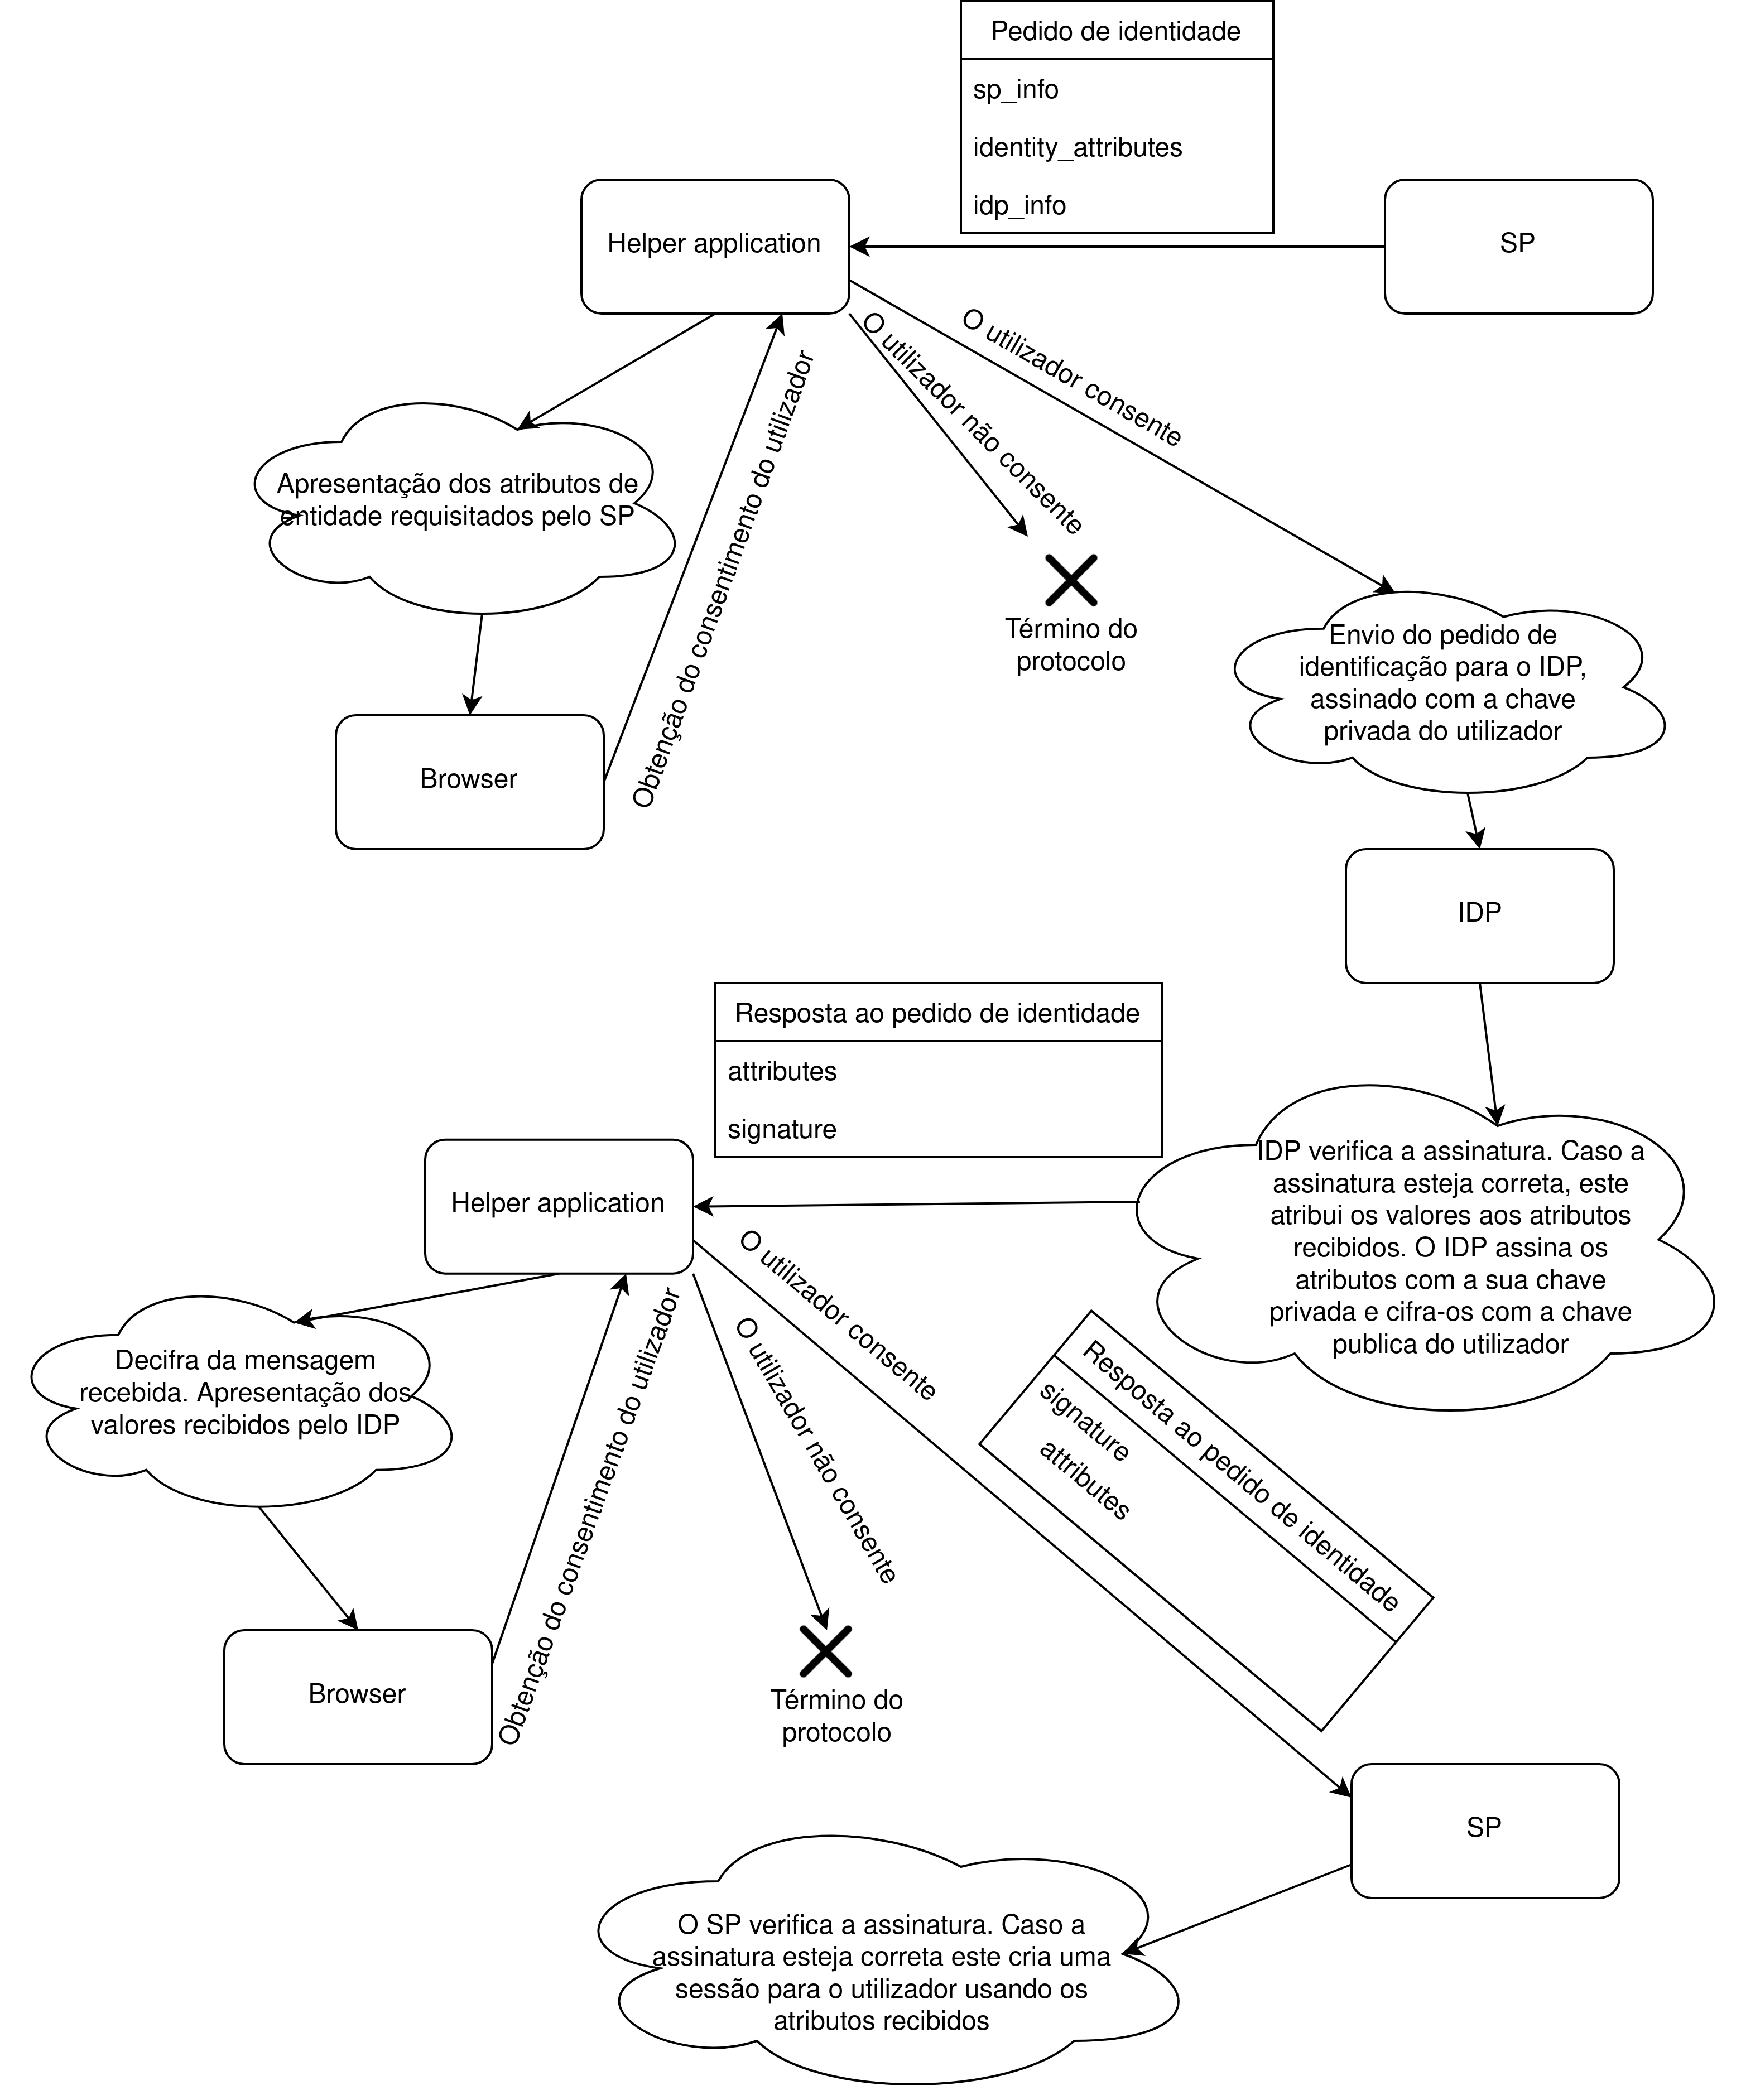
\includegraphics[width=\textwidth]{img/protocol_identity.png}
    \centering
\end{figure}


\begin{enumerate}
    \item O utilizador tenta aceder a um serviço disponibilizado por um \textit{SP} ao qual não tem uma sessão ativa, portanto, o \textit{SP} redireciona o utilizador para a \textit{helper application} enviando uma mensagem com os atributos de identidade necessários para criar uma sessão.
    \item A \textit{helper application} apresenta os atributos requisitados pelo \textit{SP} ao utilizador e obtém o consentimento do mesmo para conseguir enviar o pedido de identificação (com os atributos) para o \textit{IDP}. Obviamente, caso o utilizador não permita o uso dos atributos especificados a \textit{helper application} interrompe o processo e não envia o pedido para o \textit{IDP} \footnote{Neste fase é considerado que já existe um par de chaves assimétricas, caso estas não existam o utilizador deve ser autenticado com o protocolo \textit{ZKP} para de seguida serem criadas as credenciais assimétricas }
    \begin{figure}[H]
        \caption{Página mostrada pela \textit{helper application} para recolher o consentimento do utilizador antes do envio do pedido de identificação para o \textit{IDP}}
        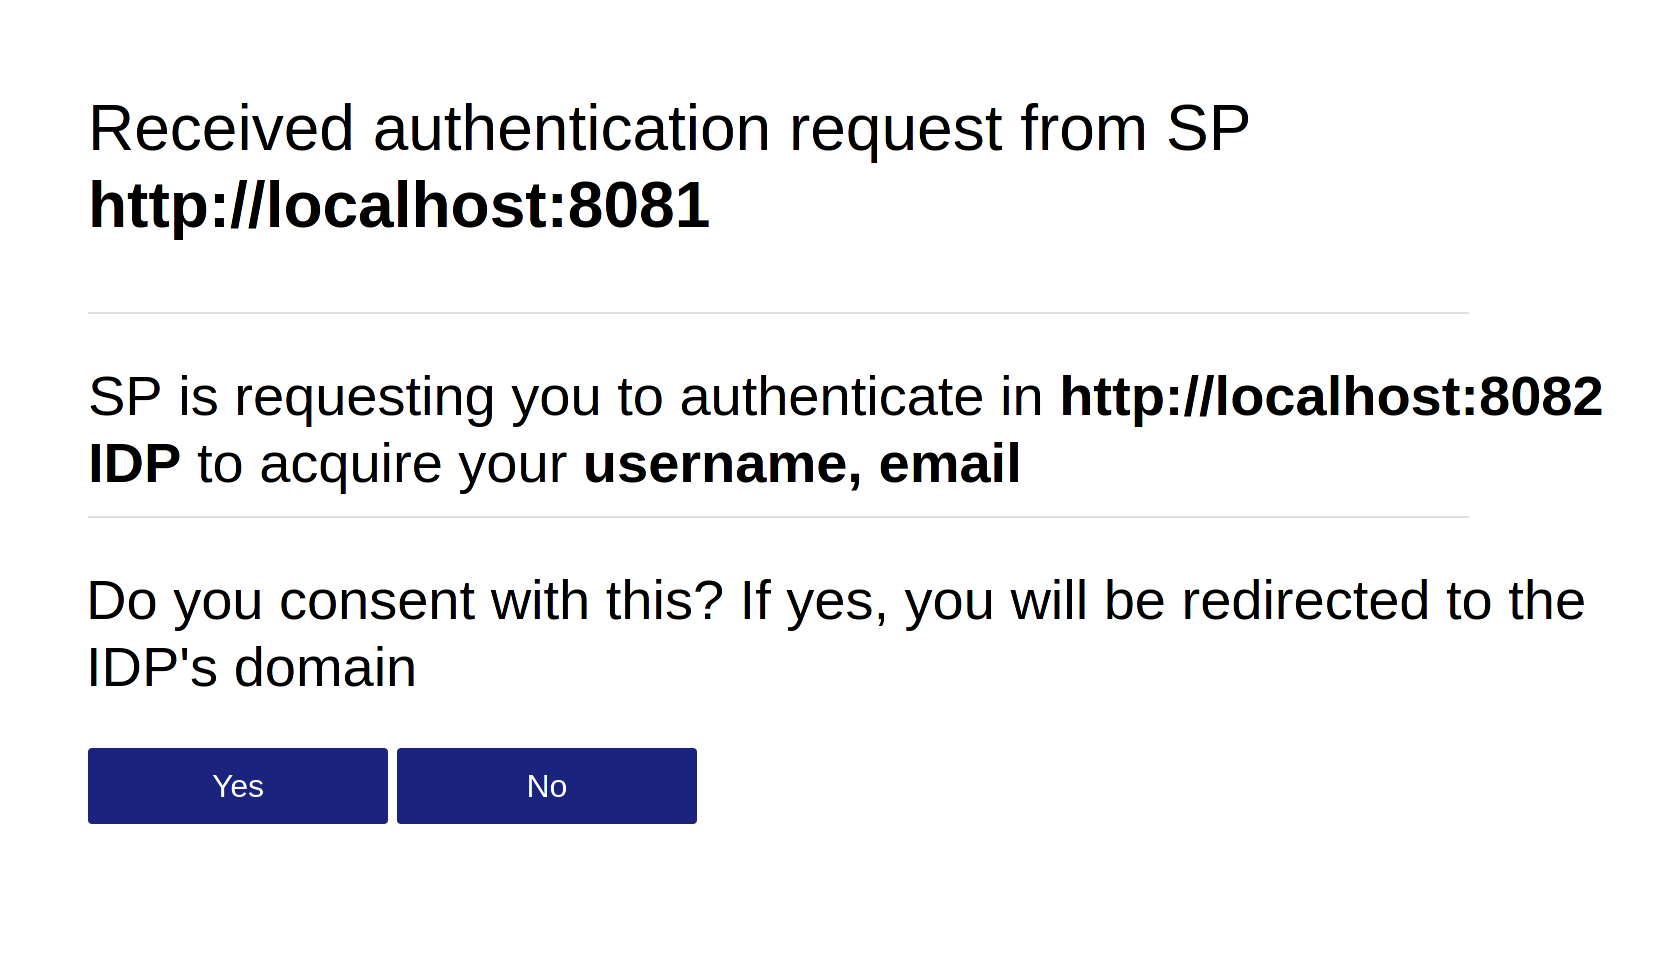
\includegraphics[width=0.6\textwidth]{img/request_conse.png}
        \centering
    \end{figure}
    \item Após receber o consentimento do utilizador a \textit{helper application} assina o pedido (usando a chave privada do utilizador, criada após o processo do \textit{ZKP}) de identificação (enviado pelo \textit{SP}) e envia o pedido e assinatura para o \textit{IDP}
    \item O \textit{IDP} após receber a mensagem anterior, este verifica a assinatura com o conteúdo recebido. Caso a assinatura seja válida este sabe que a mensagem veio do utilizador pretendido e que o conteúdo da mensagem não foi adulterado (daí o termo \textit{protocolo collapsing} pois permite numa verificação autenticar o utilizador e garantir que os dados não foram alterados no canal de comunicação). Depois da verificação da assinatura, o \textit{IDP} obtém os atributos necessários e encapsula-os numa nova mensagem com o mapeamento entre os atributos recebidos e os valores obtidos. Antes de enviar a resposta para a \textit{helper application} este faz uma assinatura sobre os conteúdos mapeados (com a chave privada associado ao \textit{IDP}) e cifra o conteúdo da mensagem com a chave publica do utilizador.
    \item A \textit{helper application} faz o processo de decifra (usando a chave privada do utilizador) da resposta recebida e apresenta ao utilizador os valores retornados pelo \textit{IDP}. Mais uma vez, obtém o consentimentos (ou não) do utilizador e caso este permita a \textit{helper application} envia o conteúdo da resposta e a respetiva assinatura para o \textit{SP}. Mais uma vez, caso não existe consentimento por parte do utilizador o processo é interrompido.
    \begin{figure}[H]
        \caption{Página mostrada pela \textit{helper application} para recolher o consentimento do utilizador antes do envio da resposta para o \textit{SP}}
        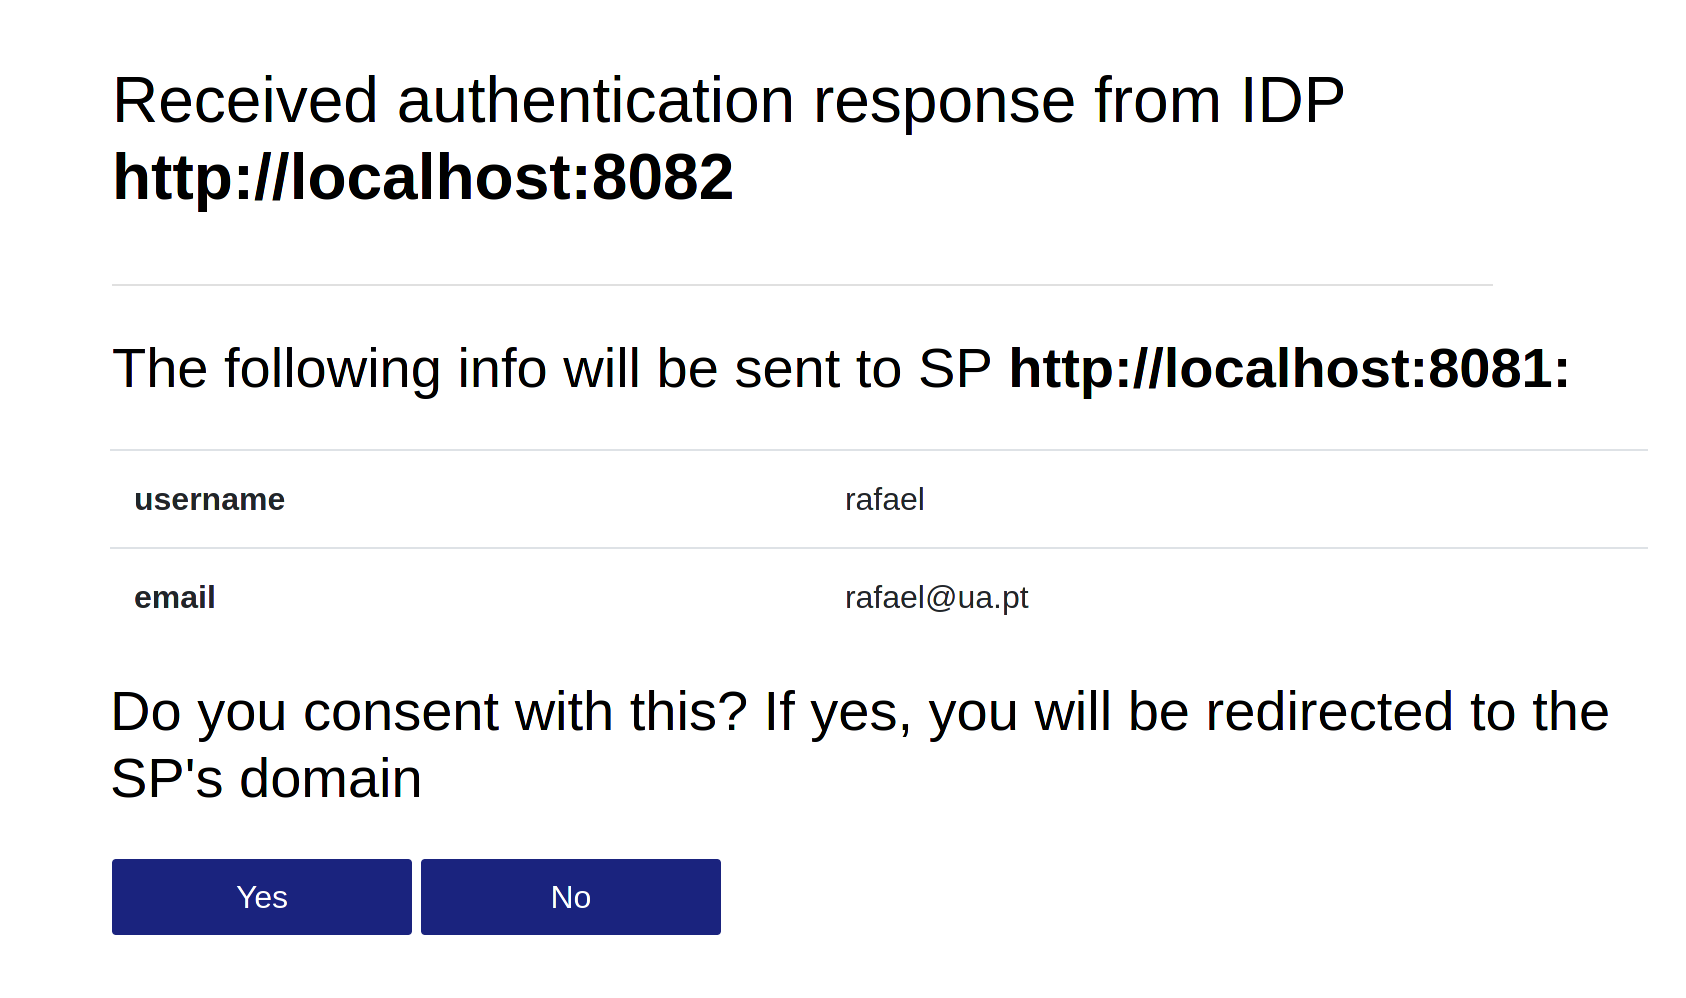
\includegraphics[width=0.6\textwidth]{img/response_conset.png}
        \centering
    \end{figure}
    \item Por fim, o \textit{SP} verifica a assinatura recebida com a chave publica do IDP e caso esta assinatura seja valida este consegue criar uma sessão para o utilizador usando os valores presentes na resposta recebida.
\end{enumerate}
